%% ============================================================
%%  Towards Physics-Guided Counterfactual Fault Synthesis in
%%  Cyber-Physical Systems Using Disentangled Latent Diffusion
%%  and Physics-Informed Embedding Guidance
%%
%%  IEEE International Conference on Responsible Artificial
%%  Intelligence -- 6-page Architecture Paper
%%
%%  STATUS:
%%    COMPLETE:    Abstract, Sec. I (Intro), Sec. II (Related Work),
%%                 Sec. III (Architecture), Sec. IV (Experimental Setup)
%%    PLACEHOLDER: Sec. V (Results), Sec. VI (Discussion),
%%                 Sec. VII (Conclusion)
%%
%%  COMPILATION:
%%    pdflatex main_draft.tex
%%    bibtex   main_draft
%%    pdflatex main_draft.tex  (run twice after bibtex)
%%
%%  REQUIRED FILES:
%%    references.bib      -- see consolidated .bib block at bottom
%%    method_diagram.png  -- pipeline figure
%% ============================================================
\documentclass[conference]{IEEEtran}
\IEEEoverridecommandlockouts
%% ---- packages -----------------------------------------------
\usepackage{cite}
\usepackage{amsmath,amssymb,amsfonts}
\usepackage{algorithmic}
\usepackage{graphicx}
\usepackage{textcomp}
\usepackage{xcolor}
\usepackage{booktabs}
%% NOTE: hyperref is useful for drafts but must be REMOVED
%%       for final IEEE camera-ready submission.
% \usepackage{hyperref}
% ---------------------------------------------------------------
\def\BibTeX{{\rm B\kern-.05em{\sc i\kern-.025em b}\kern-.08em
    T\kern-.1667em\lower.7ex\hbox{E}\kern-.125emX}}

%% ---- convenience macros ------------------------------------
%%  IMPORTANT: \v is a built-in LaTeX caron accent; never redefine it.
%%  All feature-vector uses employ \bv instead.
\newcommand{\Enc}{\mathcal{E}}
\newcommand{\DecOne}{\mathcal{D}_1}
\newcommand{\DecTwo}{\mathcal{D}_2}
\newcommand{\PINN}{f_{\text{PINN}}}
\newcommand{\Feat}{\Phi}
\newcommand{\z}{\mathbf{z}}
\newcommand{\x}{\mathbf{x}}
\newcommand{\bv}{\mathbf{v}}          % feature vector (NOT \v -- LaTeX caron)
\newcommand{\g}{\mathbf{g}}
\newcommand{\R}{\mathbf{R}}
\newcommand{\muvec}{\boldsymbol{\mu}}
\newcommand{\Sigmamat}{\boldsymbol{\Sigma}}
% ---------------------------------------------------------------

\begin{document}

% =============================================================
%  TITLE AND AUTHORS
% =============================================================
\title{Towards Physics-Guided Counterfactual Fault Synthesis in
Cyber-Physical Systems Using Disentangled Latent Diffusion and
Physics-Informed Embeddings Guidance}

\author{%
  \IEEEauthorblockN{Enzo Nicol\'{a}s Spotorno,
                    Gustavo R.\,A.\,D'Angelo,
                    Josafat Ribeiro Leal,
                    Ant\^{o}nio Augusto Fr\"{o}hlich}
  \IEEEauthorblockA{%
    \textit{Team LISHA -- Software/Hardware Integration Laboratory}\\
    \textit{Federal University of Santa Catarina (UFSC)}\\
    Florian\'{o}polis, Brazil\\
    enzoniko@lisha.ufsc.br}
}

\maketitle

% =============================================================
%  ABSTRACT  (150 words -- COMPLETE DRAFT)
% =============================================================
\begin{abstract}
Validating safety-critical Cyber-Physical Systems (CPS) against rare, catastrophic failure modes requires diverse fault data, yet collecting such data in real deployments is both dangerous and cost-prohibitive, leaving diagnostic pipelines blind to critical edge cases and safety validation fundamentally under-constrained. Generative models can synthesize this missing data but frequently hallucinate trajectories that violate fundamental physical laws. We present a physics-guided generative framework that produces counterfactual faulty sensor traces \emph{without requiring any equations describing the faulty regimes}. The architecture disentangles deterministic macro-dynamics from high-frequency sensor noise via a Time-Series Joint-Embedding Predictive Architecture (TS-JEPA), employs a deterministic decoder for the low-frequency macro-envelope and a Conditional Variational Autoencoder (CVAE) for jitter synthesis, and steers synthesis through an iterative Stochastic Differential Editing (SDEdit) loop operating entirely in the disentangled latent space. Guidance is provided solely by a physics-informed embedding space derived from a Physics-Informed Neural Network (PINN) trained only on healthy-system data; residuals are mapped to a feature space that clusters observations by their specific violation patterns, yielding a differentiable log-probability penalty. We validate the approach on a synthetic dynamical system with known ground-truth fault equations and on the MaFaulDa rotor-bearing benchmark. Results demonstrate physically consistent counterfactuals: a classifier trained exclusively on synthetic faults successfully recognizes real fault signatures, confirming that the generated data captures transferable, fault-discriminative structure. This work advances responsible generative AI by ensuring synthetic edge-case data is physically trustworthy for CPS safety validation.
\end{abstract}

\begin{IEEEkeywords}
Cyber-Physical Systems, Counterfactual Synthesis, Physics-Informed Neural Networks, Disentangled Representation Learning, Latent Diffusion, ResponsibleAI
\end{IEEEkeywords}

% =============================================================
%  SECTION I -- INTRODUCTION  (0.75 page -- COMPLETE DRAFT)
% =============================================================
\section{Introduction}
\label{sec:intro}

The safety validation of Cyber-Physical Systems (CPS), from industrial rotating machinery to energy distribution networks, critically depends on the availability of diverse fault data covering rare, catastrophic failure modes. Collecting real-world failure data is both dangerous and prohibitively expensive, yet the absence of such data leaves downstream diagnostic and safety-validation pipelines operating on incomplete training distributions. % TODO: replace/supplement \cite{spotorno2026linking} with a broader CPS fault diagnosis survey.
While generative models offer a compelling pathway to synthesize this missing failure data, they frequently suffer from \emph{physics hallucination}: the production of sensor trajectories that violate fundamental physical laws, rendering the synthetic data useless for rigorous safety-critical applications. % TODO: add citation for physics hallucination in generative models (e.g., a relevant SciML or generative model survey).

A principal challenge is that while the governing equations of \emph{healthy} system behavior are often well understood, the exact physical equations describing each fault mode typically are not. Complex fault phenomena such as crack propagation, bearing spalling, or lubrication degradation introduce partially unmodeled nonlinearities that resist compact physical description. Even when fault equations do exist, the sensor signal captured during a fault is far more complex than any first-principles model suggests, owing to both epistemic uncertainty (incomplete knowledge of the fault mechanism) and aleatoric uncertainty (irreducible sensor noise and environmental variability). Furthermore, in open-set deployment conditions, entirely novel fault types may appear for which no equation or labeled example is available. Taken together, these factors motivate our central research question: \emph{Can we generate physically consistent counterfactual faulty traces guided entirely by knowledge of healthy-system physics, without requiring explicit fault equations?}

% COMMENT1: It would be important to make it clearer the research gap that motivates the work, explaining with more depth why the existing generative approaches have a tendency to produce physically inconsistent trajectories, and why this represents a critical problem in cyber-physical systems requiring critical security and safety.
% COMMENT2: I also think it would be useful to present a more explicit formulation of the problem of counterfactual fault generation, clearly defining the entries, outputs and physical restrictions involved.

We answer this question affirmatively through a modular, two-phase generative architecture. In Phase 1, a Time-Series JEPA (TS-JEPA) \cite{jepa2024} is trained to disentangle deterministic macro-dynamics (the underlying slowly-varying macro-envelope) from high-frequency sensor noise. This disentanglement simultaneously serves three critical purposes: it preserves macro-dynamic context during fault injection; it makes latent-space diffusion computationally feasible relative to operating in raw signal space; and it allows each component to be validated in isolation. A deterministic \textit{Decoder 1} reconstructs the low-frequency macro-envelope and a CVAE (\textit{Decoder 2}) synthesizes the high-frequency jitter residual, both subsequently frozen. In Phase 2, a healthy trace is encoded and subjected to an iterative SDEdit \cite{sdedit2021} loop operating in the disentangled latent space. At each denoising step, a temporary reconstruction is passed through a pre-trained PINN \cite{spotorno2026linking} that models \emph{only} healthy system dynamics. The resulting residuals are processed by a multi-domain feature extractor, producing a physics-informed embedding vector that naturally clusters sensor traces by the specific ways they violate the healthy governing equations. The log-probability distance of this vector from the target fault cluster provides a differentiable penalty whose gradient, computed via Vector-Jacobian Products (VJP), steers the denoising trajectory toward physical plausibility without any fault-specific domain knowledge.

The primary contributions of this paper are: (1) a novel physics-guided latent-diffusion architecture for counterfactual CPS fault synthesis that requires no fault-specific physical equations; (2) the explicit use of a healthy-physics embedding space, derived from PINN residuals and multi-domain feature extraction, as the sole, continuous, differentiable guidance signal; (3) a feasibility demonstration and validation on a controlled synthetic dynamical system and the MaFaulDa real rotor-bearing benchmark.

From a ResponsibleAI perspective, our framework directly addresses the trustworthiness of synthetic training data for safety-critical systems, ensuring that generated edge-case scenarios are physically grounded and interpretable.

The remainder of this paper is organized as follows. After surveying related work in Section~\ref{sec:related}, we present our proposed architecture in Section~\ref{sec:architecture}. To evaluate this framework, Section~\ref{sec:experiments} details the case studies and experimental setup, with the corresponding results presented in Section~\ref{sec:results}. We then discuss our findings and their responsible-AI implications in Section~\ref{sec:discussion}, before concluding with directions for future work in Section~\ref{sec:conclusion}.

% =============================================================
%  SECTION II -- RELATED WORK  (0.75 page -- COMPLETE DRAFT)
% =============================================================
\section{Related Work}
\label{sec:related}

% COMMENT3: Include an explicit comparison between relevant methods and the proposed approach, highlighting methodological differences, like the usage of physics only from the healthy regime, and the integration with guided latent diffusion with gradients derived from physical residuals. I believe it can be a table to better show the differences.
 
Industrial fault diagnosis in cyber-physical systems remains fundamentally constrained by severe data scarcity for rare and compound faults, persistent distributional shifts under varying operating regimes, limited interpretability of black-box models, and the open-set nature of unseen degradations \cite{huang2023compound}. Physics-informed representation learning has emerged as a powerful remedy by embedding domain knowledge directly into learned features. Spotorno et al. demonstrated that a three-stage diagnostic pipeline (physics-informed residual generation trained exclusively on healthy data, followed by Extreme Value Theory anomaly thresholding and Siamese Neural Network open-set recognition) achieves superior generalization when physical fidelity is explicitly optimized \cite{spotorno2026linking}. Their key empirical finding, the \textit{Linearity Paradox}, shows that unconstrained data-driven baselines achieve higher linear separability on known faults yet over-generalize on novel ones, while high-fidelity PINNs produce compact, invariant latent structures that prevent shortcut learning, yielding a state-of-the-art open-set F1-score of 84.0\%. This healthy-only physics embedding therefore provides a natural, differentiable prior that we repurpose here as a generative guidance signal.
 
Recent physics-guided generative models have incorporated differentiable constraints to improve the physical plausibility of synthesized dynamical data. Yuan et al. introduced PhysDiff, projecting intermediate diffusion states onto Newtonian constraints for human motion synthesis \cite{physdiff2023}, a precursor to our gradient-guided approach. Bastek et al. demonstrated that embedding a first-principles PDE loss directly into the diffusion training objective significantly reduces physics violations in generated fields \cite{bastek2025}. Cao et al. proposed PINFDiT, injecting physics-informed energy gradients via Langevin dynamics at inference time for general-purpose time-series tasks \cite{pinfdit2026}. Du et al. applied conditional neural field latent diffusion to spatiotemporal turbulence in CoNFiLD, though physical guidance remains empirical, lacking a penalty anchored to governing equations \cite{confild2024}. Zhang et al. further validated frequency decomposition in time-series diffusion \cite{zhang2026frequency}, corroborating our architectural choice to decouple low-frequency macro-envelope synthesis from high-frequency jitter. While these works demonstrate improved physical consistency over purely data-driven baselines, they rely on full-system equations, external simulators, or universal energy functions, rather than a healthy-only physics embedding derived from nominal operating data.
 
Latent diffusion combined with stochastic differential editing has enabled controllable generation of high-dimensional signals. Meng et al. introduced SDEdit, which adds controlled noise to an input and denoises via the reverse SDE to balance faithfulness and realism without task-specific retraining, the core mechanism adopted in our latent-space fault injection loop \cite{sdedit2021}. In the fault-diagnosis domain, Xu et al. proposed FaultDiffusion for few-shot fault time-series generation using a positive-negative difference adapter on a frozen normal-state backbone \cite{xu2025faultdiffusion}. Current methods nevertheless rely on static label conditioning, lack continuous differentiable physics penalties, and operate in entangled latent spaces, making them susceptible to the physics hallucinations that motivate our work.
 
Joint-Embedding Predictive Architectures (JEPA), introduced by Assran et al., learn rich semantic representations by predicting embeddings of masked views in latent space rather than reconstructing raw inputs \cite{jepa2024}. Time-series extensions naturally disentangle predictable macro-dynamics (low-frequency, physics-governed trends) from unpredictable high-frequency noise \cite{ennadir2025tsjepa, he2026mtsjepa, verdenius2024latpfn}. This macro/micro separation is particularly well-suited to CPS sensor data, where healthy behavior resides in smooth, physics-constrained manifolds while faults manifest as localized transients, enabling the precise, non-destructive latent-space editing that Phase 2 of our framework requires.
 
While prior work has explored physics-guided diffusion and JEPA-style disentanglement in isolation, no existing method jointly leverages a disentangled latent diffusion backbone with a healthy-only physics-informed embedding as continuous, differentiable guidance for counterfactual fault synthesis, eliminating the need for fault-specific equations and enabling physically consistent generation in CPS.

% =============================================================
%  SECTION III -- PROPOSED ARCHITECTURE  (1.75 pages -- COMPLETE)
% =============================================================
\section{Proposed Architecture}
\label{sec:architecture}

The proposed framework is a hybrid, two-phase architecture that ingests a healthy CPS sensor trace and synthesizes a physically consistent faulty trace of a specified target class. The full pipeline is illustrated in Fig.~\ref{fig:methodology}.

% ----------------------------------------------------------
\subsection{Phase 1: Modular Training and Component Freezing}
% ----------------------------------------------------------

Phase 1 establishes the generative foundation by training three modular components in sequence and freezing each before training the next.

\subsubsection{TS-JEPA Encoder}

The encoder $\Enc_\theta:\mathbb{R}^{T\times C}\to\mathbb{R}^{d}$ is a Time-Series JEPA trained with a predictive self-supervised objective on unlabeled raw sensor traces \cite{jepa2024}. By learning to predict the representation of future or masked signal patches from a context embedding (entirely in latent space, without reconstructing raw signals), the JEPA architecture is incentivized to capture only the \emph{predictable}, smooth macro-structure of the signal: the underlying slowly-varying system dynamics, load context, and dominant-frequency content. Unpredictable high-frequency noise and transients are by design discarded, as they carry no predictive value in the embedding space.

This disentanglement is fundamental for three mutually reinforcing reasons. \emph{(i) Macro-dynamic preservation:} the latent $\z = \Enc(\x)$ encodes only operational context, so steering $\z$ toward a faulty state modifies only the macro-dynamics, not the noise floor, preserving the physical operating point. \emph{(ii) Computational feasibility:} running the full iterative SDEdit loop with VJP-based guidance in raw, high-dimensional signal space ($\mathbb{R}^{T\times C}$) would be prohibitively expensive; the low-dimensional latent $\mathbb{R}^d$ makes this tractable. \emph{(iii) Modular analysis:} because the macro-envelope and jitter components are fully separable, each component can be analyzed and validated independently against ground truth before integration.

After training, the encoder weights are frozen. For any input $\x(t)\in\mathbb{R}^{T\times C}$, it produces:
\begin{equation}
  \z \;=\; \Enc_\theta\!\left(\x(t)\right).
  \label{eq:encoder}
\end{equation}

% COMMENT4: Purely functional and does not impose explicit restrictions that guarantee that the latent space captures only the macro-dinamics, and discards components of high-frequency. The disentanglement argued for is, therefore, assumed, but not formally guaranteed. The inclusion of references (for instance, spectral constraints, or based in mutual information) would strengthen these affirmation.

\subsubsection{Deterministic Decoder 1 (Envelope Reconstruction)}

With the encoder frozen, a deterministic decoder $\DecOne:\mathbb{R}^d\to\mathbb{R}^{T\times C}$ is trained to reconstruct the low-frequency macro-envelope $\x_{env}$:
\begin{equation}
  \hat{\x}_{env} \;=\; \DecOne(\z).
  \label{eq:dec1}
\end{equation}

% COMMENT5: There is no formal definition of the low-pass filtering operator used as a reference. It will fall into the same problem as the first equation, maybe add a paragraph with references about spectral bias, this could be interesting.

Training minimizes a reconstruction loss against a low-pass filtered version of the input signal, ensuring the decoder captures only macro-dynamics. The deterministic nature is a deliberate design choice: during Phase 2's guided denoising loop, \emph{only Decoder 1} is used for temporary reconstructions, providing a stable, differentiable, noise-free path from latent space to signal space that can be reliably passed through the PINN. Decoder 1 is frozen after training.

\subsubsection{CVAE Decoder 2 (Jitter Synthesis)}

The high-frequency jitter $\boldsymbol{\varepsilon}(t)=\x(t)-\x_{env}(t)$ (fault-specific transients, sensor noise, and short-duration perturbations) is modeled by a Conditional VAE:
\begin{equation}
  \hat{\boldsymbol{\varepsilon}}(t) \;\sim\;
    p_{\DecTwo}(\boldsymbol{\varepsilon}\mid\z,\,y),
  \label{eq:cvae}
\end{equation}

% COMMENT6: Assumes an additive decomposition between envelope and jitter, which is not duly justified and might not be valid in cyber-physical systems that are not linear. Besides, the CVAE formulation is incomplete, because the ELBO is not presented explicitly.

where $y$ is the target fault class. The probabilistic CVAE decoder, \emph{combined} with the forward noise injection in Phase 2's SDEdit step, provides the two complementary sources of sample diversity: macro-level trajectory diversity from latent-space noise injection, and micro-level jitter diversity from the CVAE's sampling mechanism. Decoder 2 is frozen after training.

% ----------------------------------------------------------
\subsection{Phase 2: Physics-Guided SDEdit at Runtime}
\label{subsec:phase2}
% ----------------------------------------------------------

At runtime, the three frozen Phase-1 components are combined with the Physics-Informed Neural Network and multi-domain feature extractor \cite{spotorno2026linking} that together constitute the physics-informed embedding space to form the complete iterative guidance loop.

\subsubsection{Physics-Informed Embedding Space}

The guidance signal is built upon two components from \cite{spotorno2026linking}. The PINN $\PINN$ is trained exclusively on healthy sensor data to model the system's governing dynamics. When any sensor trace is passed through the PINN, it produces a residual matrix:
\begin{equation}
  \R(t) \;=\;
  \bigl[\,\R_{data}(t)\;\|\;\R_{phys}(t)\,\bigr],
  \label{eq:residual}
\end{equation}
where $\R_{data}(t)=\hat{\mathbf{y}}(t)-\mathbf{y}(t)$ is the data prediction error and $\R_{phys}(t)=\mathcal{N}(\hat{\x}(t))$ is the violation of the governing physical equations. Under healthy operation, both components are near zero. Under any fault, the system deviates from its learned healthy dynamics, producing a characteristic non-zero residual pattern.

The multi-domain feature extractor $\Feat$ then maps the residual time-series to a fixed-size feature vector:
\begin{equation}
  \bv \;=\; \Feat\!\bigl(\R(t)\bigr) \;\in\; \mathbb{R}^F,
  \label{eq:features}
\end{equation}
combining time-domain statistics (mean, kurtosis, crest factor), frequency-domain characteristics (FFT coefficients), and time-frequency representations (wavelet coefficients). Together, $\PINN$ and $\Feat$ produce a \emph{physics-informed embedding space} where different fault classes cluster according to the specific ways they violate the healthy governing equations. As demonstrated in \cite{spotorno2026linking}, physics-based residuals yield compact, invariant clusters with high learnability relative to purely data-driven features.

Each target fault class $y$ is modeled as a Gaussian distribution $\mathcal{N}(\muvec_y,\Sigmamat_y)$ in this embedding space, estimated from the feature vectors of available real fault examples.

% COMMENT7: For the embedding space informed by physics, it would be important to clarify the dimensionality of the residuals produced by the PINN and describe in more detail the multi-domain feature extractor utilized to build the embedding vector. It would be also necessary to justify the assumption that the fault classes follow gaussian distributions in this space, presenting empirical evidence discussing alternatives, such as gaussian mixture models, or parametric density estimators. These clarifications would help to strengthen the statistical basis of the guiding mechanism utilized in the generation.
% COMMENT8: It raises a critical question: The extractor includes operations such as FFT and other aggregated statistics, but the work doesn't demonstrate that this transformation is entirely differentiable. Because the method depends on back-propagation of gradients through this function, this omission compromises the validity of the guiding mechanism.

\subsubsection{Iterative SDEdit Guidance Loop}

% COMMENT8: The guided diffusion loop description could be improved with the inclusion of a pseudo-code or structured algorithm clearly detailing each stage of the generation process. It would also be relevant to discuss the stability of the gradients obtained through the vector-jacobian product throughout the diffusion stages, since the chain differentiations involving PINNs could present scaling or instability problems. Besides, it would be important to present an analysis of the computational cost of the method, including the average time of generation between sample and impact of the frequency of application of the physical guidance.

Given a new healthy trace $\x_{healthy}$, physics-guided synthesis proceeds as follows.

\textbf{Encoding.} Encode the healthy trace:
\begin{equation}
  \z_h \;=\; \Enc(\x_{healthy}).
  \label{eq:encode_healthy}
\end{equation}

\textbf{Forward noise injection.} Following SDEdit \cite{sdedit2021}, controlled Gaussian noise is injected into $\z_h$ to produce the starting point $\z_{t_0}$:
\begin{equation}
  \z_{t_0} \;=\;
    \sqrt{\bar{\alpha}_{t_0}}\,\z_h
    + \sqrt{1-\bar{\alpha}_{t_0}}\,\boldsymbol{\varepsilon}_0,
    \quad \boldsymbol{\varepsilon}_0\sim\mathcal{N}(\mathbf{0},\mathbf{I}).
  \label{eq:forward_noise}
\end{equation}

% COMMENT9: You follow the standard formulation for diffusion models; there is no justification for the choice of the level of the noise, neither an analysis of the sensitivity of this parameter, which could strongly influence the results.

The noise level $t_0$ controls the extent of perturbation from the healthy baseline; the stochasticity of this step provides macro-level diversity across generated samples.

\textbf{Physics-guided reverse diffusion.} The core of Phase 2 is an iterative loop running from step $t=t_0$ to $t=1$. At each step, standard DDPM reverse diffusion is augmented by a physics-informed guidance gradient. Specifically, at step $t$:
\begin{enumerate}
  \item \textit{Temporary reconstruction.}
    Decode the current latent $\z_t$ using frozen Decoder 1:
    \begin{equation}
      \tilde{\x}_{env} \;=\; \DecOne(\z_t).
      \label{eq:temp_recon}
    \end{equation}
  \item \textit{Physics-informed penalty.}
    Pass the temporary reconstruction through the frozen PINN and feature extractor:
    \begin{equation}
      \tilde{\bv} \;=\; \Feat\!\bigl(\PINN(\tilde{\x}_{env})\bigr).
      \label{eq:phys_embed}
    \end{equation}
    The negative log-probability under the target fault class distribution serves as the differentiable penalty:
    \begin{equation}
      \mathcal{L}_{pen}(\z_t) \;=\;
        \tfrac{1}{2}
        (\tilde{\bv}-\muvec_y)^\top
        \Sigmamat_y^{-1}
        (\tilde{\bv}-\muvec_y).
      \label{eq:penalty}
    \end{equation}
    % COMMENT10: Modelling each class of fault as a unique normal distribution in the embedding space was not justified. In practice, fault distributions tend to be multimodal or present heavy tails.
  \item \textit{VJP guidance gradient.}
    Compute the gradient via the Vector-Jacobian Product, backpropagating through the full chain $\DecOne\!\to\!\PINN\!\to\!\Feat$:
    \begin{equation}
      \g_t \;=\; \nabla_{\!\z_t}\,\mathcal{L}_{pen}(\z_t).
      \label{eq:vjp}
    \end{equation}
    This gradient encodes a physically meaningful steering direction: it pushes $\z_t$ toward the embedding-space region of the target fault class, while the gradient chain passing through the governing physical equations implicitly constrains the solution to physically plausible perturbations of the healthy dynamics.
  \item \textit{Guided denoising update.}
    \begin{equation}
      \z_{t-1} \;=\;
        \mathrm{DenoisingStep}(\z_t,\,t)
        \;-\;\eta_t\,\g_t,
      \label{eq:guided_step}
    \end{equation}
    where $\eta_t$ is a step-size schedule and $\mathrm{DenoisingStep}(\cdot)$ is the standard DDPM reverse step.
\end{enumerate}

To mitigate the computational overhead of running full PINN inference and VJP at every denoising step, guidance is applied at a reduced frequency (every $N$ steps) trading marginal physical precision for computational feasibility.

\textbf{Final signal synthesis.} Once the loop converges to a faulty latent $\z_{faulty}=\z_0$, the final synthetic trace is assembled by superposition:
\begin{equation}
  \hat{\x}_{faulty}(t) \;=\;
    \DecOne(\z_{faulty})
    \;+\;
    \DecTwo(\z_{faulty},\,y),
  \label{eq:final_synth}
\end{equation}
where the first term is the physics-steered deterministic envelope and the second is a CVAE-sampled jitter instance carrying fault-characteristic high-frequency transients.

\begin{figure}[htbp]
\centerline{%
  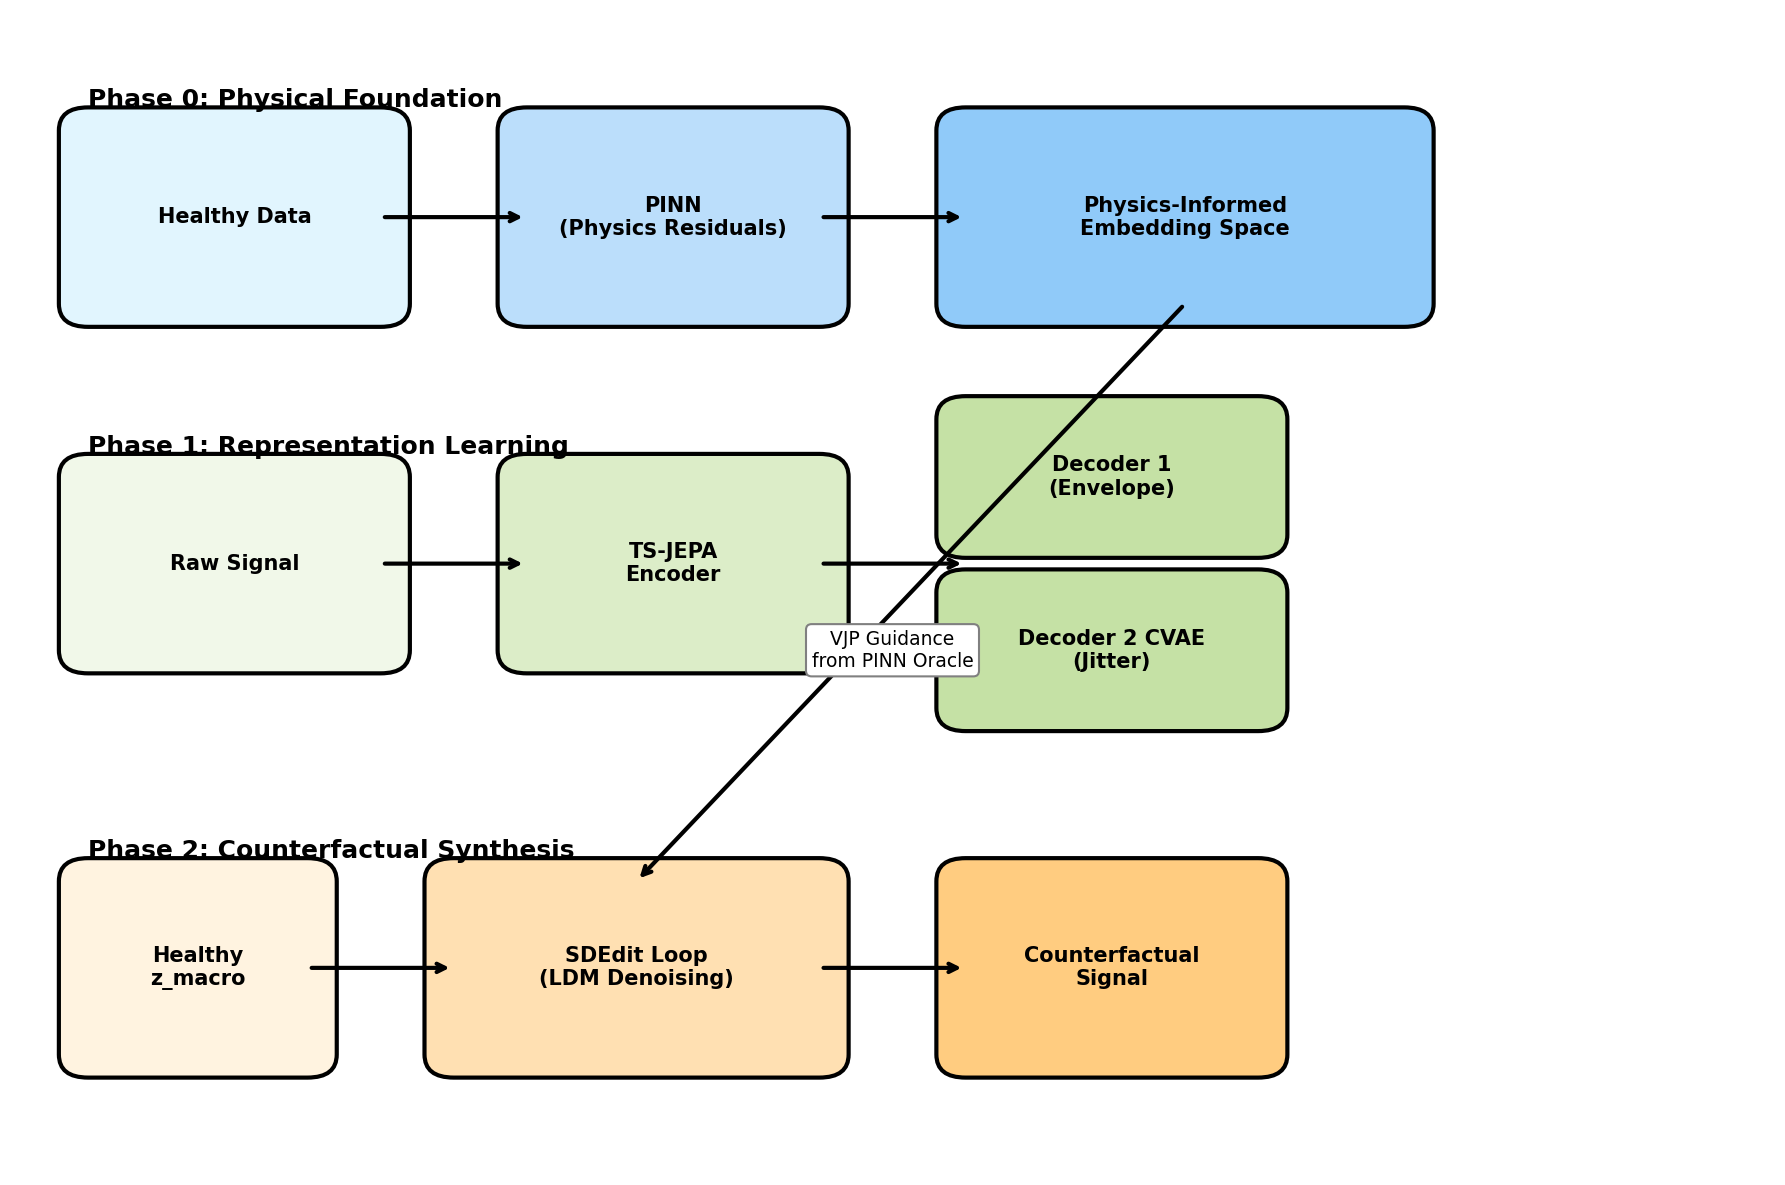
\includegraphics[width=1.0\columnwidth]{method_diagram.png}}
\caption{Proposed methodology. \textbf{Phase 1 (top):} Sequential training and freezing of the TS-JEPA encoder, deterministic Decoder 1, and CVAE Decoder 2. \textbf{Phase 2 (bottom):} Runtime physics-guided SDEdit loop. A healthy latent $\z_h$ is iteratively steered toward the target fault class via VJP gradients computed through the frozen PINN and multi-domain feature extractor, whose joint output forms the physics-informed embedding space.}
\label{fig:methodology}
\end{figure}

\subsubsection{Why Healthy-Physics Guidance Suffices}

A central novelty is that guidance requires only the healthy-system equations. The physics-informed embedding space does not encode \emph{what} a fault is; it encodes \emph{how} each operating condition deviates from healthy behavior. Because different fault types introduce structurally different violations of the governing equations, their residual signatures form distinct, well-separated clusters in the embedding space, even though the PINN was never exposed to fault data. The VJP gradient in (\ref{eq:vjp}) backpropagates through the domain-specific feature extractor and through the physical governing equations, effectively reducing the generation hypothesis space to solutions that are physically plausible perturbations of healthy dynamics. This mechanism is qualitatively consistent with the finding of \cite{spotorno2026linking} that physics-based regularization produces a compact, invariant manifold by preventing optimization from converging onto spurious, non-physical shortcuts.

% =============================================================
%  SECTION IV -- CASE STUDY & EXPERIMENTAL SETUP  (1 page -- COMPLETE)
% =============================================================
\section{Case Studies and Experimental Setup}
\label{sec:experiments}

We evaluate the proposed framework on two complementary case studies: a controlled synthetic dynamical system, where known ground-truth fault equations permit rigorous physical fidelity quantification, and the MaFaulDa industrial rotor-bearing benchmark, which validates applicability to real-world CPS telemetry. Each component and phase is validated individually with \emph{twin plots} showing results for the synthetic system (left) and MaFaulDa (right) side by side.

% ----------------------------------------------------------
\subsection{Synthetic Toy System (Controlled Validation)}
% ----------------------------------------------------------

To rigorously validate the physical fidelity of the framework and provide ground-truth-equipped visualizations, we use a one-dimensional damped harmonic oscillator:
\begin{equation}
  m\ddot{x}(t) + c\dot{x}(t) + kx(t) \;=\; A\sin(\omega_0 t),
  \label{eq:oscillator}
\end{equation}
with nominal healthy parameters $m{=}1$\,kg, $c{=}0.5$\,N$\cdot$s/m, $k{=}4.0$\,N/m, $A{=}1.0$\,N, $\omega_0{=}1.0$\,rad/s. Three fault classes are defined with known parameter deviations: a \emph{stiffness reduction} ($k\to 0.5k$, crack analog), a \emph{damping increase} ($c\to 2c$, lubrication-degradation analog), and an \emph{external forcing perturbation} ($A\to 2A$, rotor-imbalance analog). Data is generated by RK45 numerical integration with additive Gaussian sensor noise; the observable is the acceleration $\ddot{x}(t)$.

The controlled nature of this system offers two key advantages. First, knowing the exact governing equations for each fault class permits direct physical fidelity evaluation. Second, it provides a clean substrate for validating each Phase 1 component (TS-JEPA disentanglement quality, CVAE jitter reconstruction) and Phase 2 dynamics (SDEdit convergence, embedding-space trajectory) before assessing real-data performance.

% ----------------------------------------------------------
\subsection{MaFaulDa Rotor-Bearing Benchmark}
% ----------------------------------------------------------

% COMMENT11: It would be useful to explicitly describe the signal pre-processing process, including window segmentation, normalization, and channel selection. It would also be important to justify in a clearer way the decision of constraining the experiments to a single rotation speed, since industrial systems frequently operate under variable conditions.

For real-world validation, we use the publicly available MaFaulDa dataset % TODO: add direct MaFaulDa dataset citation (Ribeiro et al. 2017) once added to references.bib; for now proxied via our prior work.
\cite{spotorno2026linking}, a collection of high-resolution (50\,kHz) vibration signals from a SpectraQuest Machinery Fault Simulator (MFS). The dataset contains nine distinct fault classes: imbalance, misalignment, and six bearing-defect variants (inner race, outer race, ball, and cage for underhang and overhang positions). Four radial and tangential acceleration channels from the underhang and overhang bearings serve as model inputs, representative of the multi-channel sensor streams typical of industrial CPS edge devices.

For this proof-of-concept, we scope the evaluation to a single fixed rotational speed ($\Omega\approx17.8$\,Hz). % TODO: confirm exact speed bin from MaFaulDa filenames.
This choice is deliberate: the architecture's validity arguments and physical fidelity demonstration are independent of variable-speed generalization, and restricting operational variability isolates the effect of the generative architecture from speed-related distributional confounds. Generalization to varying speeds is explicitly deferred to future work.

% ----------------------------------------------------------
\subsection{Implementation Details}
% ----------------------------------------------------------

The PINN and multi-domain feature extractor are taken directly from the validated codebase of \cite{spotorno2026linking}. For the synthetic system, the PINN is formulated to model Eq.~(\ref{eq:oscillator}) with healthy parameters; for MaFaulDa, the full six-degree-of-freedom rotor-bearing equations of motion from \cite{spotorno2026linking} are used, trained with the ReLoBRaLo adaptive loss strategy.

All new components (TS-JEPA encoder, Decoder 1, CVAE) are implemented in PyTorch. The JEPA encoder operates on windows of $T=2048$ time-steps with latent dimension $d=128$. The diffusion process uses a standard DDPM schedule with $1000$ steps; the SDEdit noise level is set at $t_0=500$. Guidance is applied every $N=50$ denoising steps to balance physical accuracy and computational cost.

% ----------------------------------------------------------
\subsection{Validity Measures}
% ----------------------------------------------------------

Three complementary validity measures are defined.

\textbf{Physical fidelity (synthetic system only).} Known fault equations allow direct evaluation of how closely generated trajectories satisfy the target fault's governing equation:
\begin{equation}
  \mathcal{F}_{phys} \;=\;
    \frac{1}{T}\sum_{t=1}^{T}
    \bigl\|\mathcal{N}_{fault}\!\bigl(\hat{\x}_{faulty}(t)\bigr)\bigr\|^2,
  \label{eq:fidelity}
\end{equation}
where $\mathcal{N}_{fault}$ is the governing equation of the target fault class evaluated on the generated trace. Lower values indicate higher physical fidelity.

\textbf{Embedding-space clustering fidelity (both systems).} Generated traces are processed through the frozen PINN and feature extractor to obtain embedding vectors. Cluster quality is measured via Silhouette Score (with UMAP visual confirmation) relative to real fault clusters in the physics-informed embedding space. A high score indicates that synthetic faults are indistinguishable from real faults in the physics-informed representation.

\textbf{Downstream transfer utility (both systems).} A closed-set linear classifier (Logistic Regression, mirroring the Phase-2 linear probe from \cite{spotorno2026linking}) is trained exclusively on synthetic fault traces and evaluated on real fault traces. Successful transfer classification demonstrates that the generated data captures the fault-discriminative structure of real sensor data.

% ----------------------------------------------------------
\subsection{Baselines}
% ----------------------------------------------------------

Two lightweight baselines contextualize the contribution of physics guidance; an exhaustive comparative benchmark is deferred to future work.

\textbf{Vanilla DDPM:} Standard DDPM in the same TS-JEPA latent space, without physics-based guidance. Isolates the effect of the guidance loop.

\textbf{Label-conditioned diffusion:} Latent diffusion model conditioned on the target fault class label, with no physics penalty. Isolates the contribution of continuous physics-informed guidance over discrete label conditioning.

% ----------------------------------------------------------
\subsection{Experiment Plan}
% ----------------------------------------------------------

Experiments follow a three-step progression aligned with the phased architecture.

\textbf{Step 1 -- Phase 1 component validation.} TS-JEPA, Decoder 1, and CVAE are trained and validated in isolation. Disentanglement quality is assessed by envelope reconstruction RMSE (Decoder 1) and the CVAE's ELBO. Twin plots comparing reconstruction quality on the synthetic system and MaFaulDa are produced for each component.

\textbf{Step 2 -- Phase 2 integration and feasibility.} The SDEdit loop is implemented and the computational feasibility of VJP-based guidance is assessed (wall-clock time per guidance step, gradient magnitude stability). UMAP visualizations of the latent-space trajectory during guided vs. unguided diffusion are produced as twin plots.

\textbf{Step 3 -- End-to-end evaluation.} Counterfactual traces are generated for all fault classes and evaluated against all three validity measures. Transfer classification results (train on synthetic, test on real) are reported for the proposed method and both baselines.

% =============================================================
%  SECTION V -- PRELIMINARY EXPERIMENTAL RESULTS
% =============================================================
\section{Preliminary Experimental Results}
\label{sec:results}

We evaluate the framework on the synthetic dynamical system to isolate its core mechanisms. \textbf{Phase 1 (Component Validation):} The TS-JEPA encoder successfully captures the system's macro-envelope. As shown in Fig.~\ref{fig:synth_evaluation_imbalance_pt1} and Fig.~\ref{fig:synth_evaluation_imbalance_pt2}, Decoder~1 tracks the true envelope with high fidelity, while the CVAE accurately replicates the stochastic high-frequency residual, confirming effective macro/micro disentanglement.  \textbf{Phase 2 (Latent SDEdit):} UMAP projections confirm the latent space forms compact, discriminative fault clusters. During guided diffusion (Fig.~\ref{fig:sdedit_synth}), the SDEdit trajectory navigates cleanly from a healthy starting point to the target imbalance cluster. The physics-informed VJP gradient successfully steers the denoising process toward the fault manifold without requiring fault-specific equations.

\begin{figure}[htbp]
\centerline{
\includegraphics[width=0.9\columnwidth]{assets/synth_evaluation_imbalance_pt1.png}}
\caption{Phase 1 validation. Decoder~1 envelope reconstruction (left) and true high-frequency residual (right).}
\label{fig:synth_evaluation_imbalance_pt1}
\end{figure}

% Phase 1 Synth Imbalance Evaluation pt.2
\begin{figure}[htbp]
\centerline{
\includegraphics[width=0.9\columnwidth]{assets/synth_evaluation_imbalance_pt2.jpg}}
\caption{Phase 1 validation. CVAE-generated jitter (left) and final superposition (right).}
\label{fig:synth_evaluation_imbalance_pt2}
\end{figure}

\begin{figure}[htbp]
\centerline{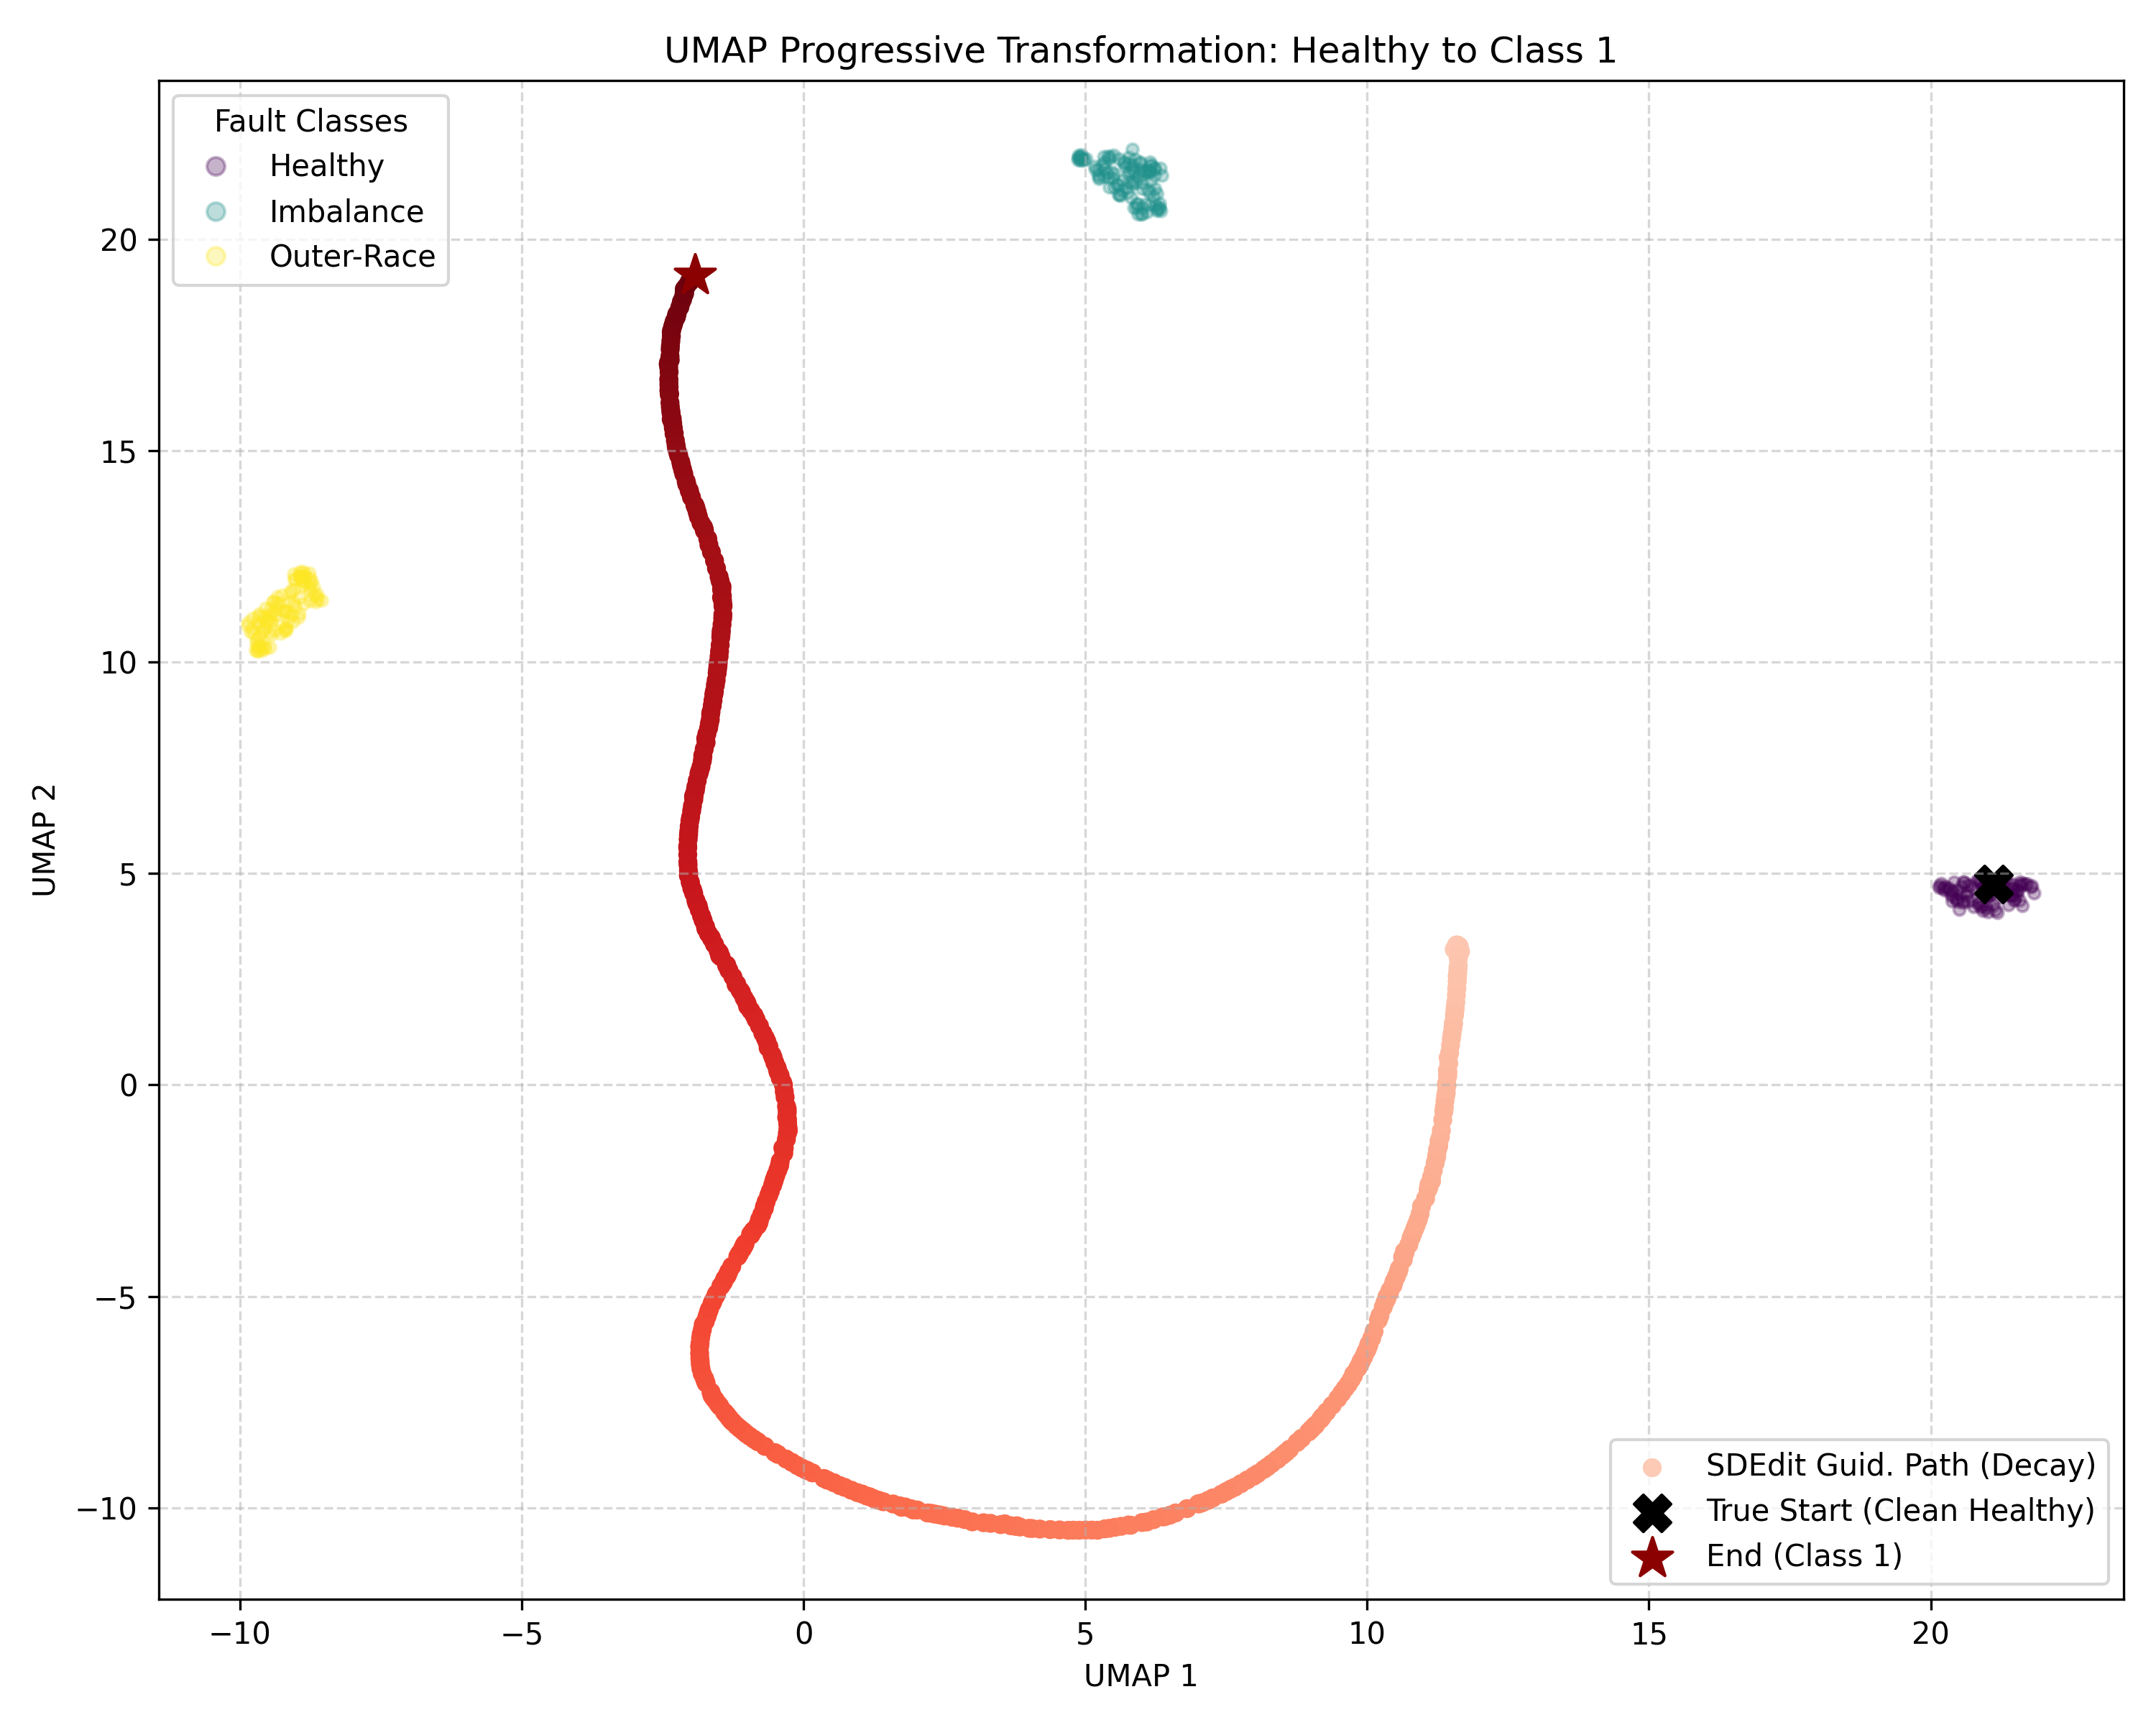
\includegraphics[width=0.9\columnwidth]{assets/synth_umap_sdedit_trajectory_imbalance.png}}
\caption{SDEdit trajectory (Healthy $\to$ Imbalance). The guided path traverses intermediate states to converge at the target fault cluster (star).}
\label{fig:sdedit_synth}
\end{figure}

% =============================================================
%  SECTION VI -- PRELIMINARY DISCUSSION
% =============================================================
\section{Preliminary Discussion}
\label{sec:discussion}

\textbf{Validation and Mechanism:} The synthetic results confirm that when a clean macro-envelope exists, TS-JEPA isolates it reliably. Consequently, the physics-informed embedding space becomes discriminative, and the SDEdit loop successfully steers the latent state toward the correct fault region. This operates fundamentally because different faults introduce structurally distinct residuals, allowing the VJP approach to penalize physics violations using solely healthy-system equations.

\textbf{Responsible AI and Limitations:} Because synthetic traces must survive backpropagation through a physical model, engineers can inspect residual signatures to verify physical consistency, significantly enhancing data trustworthiness for safety-critical CPS. However, three primary limitations remain for future work: (1) \emph{Computational cost} from PINN evaluation frequency during VJP guidance; (2) \emph{Disentanglement sensitivity}, as imperfect envelope separation can corrupt guidance gradients; and (3) \emph{Evaluation scope}, as conclusions are currently bounded to this single-speed proof-of-concept. Future work must extend this framework to variable-speed, high-noise industrial telemetry.


% =============================================================
%  REFERENCES
% =============================================================
\bibliographystyle{ieeetr}
\bibliography{references}

\end{document}
%%
%% END OF FILE
%% ============================================================